 \documentclass[book.tex]{subfiles}
\begin{document}
\chapter{Real Mode Memory Models}
\label{appendix_memory_models}

The opposite of the medium model is the compact model. Here the total function code cannot exceed 64KiB, but there is more space for global data, stack and heap. The large model can deal with function code and data larger than 64KiB, but is slow in execution as only far pointers are used for both code and data. Borland C++ limits the size of all global data to 64KiB. The huge memory model sets aside that limit, allowing global data to occupy more than 64KiB\footnote{Also here the same limitation as before: If the source file is too big to fit into one 64KiB data segment, the programmer must break it up into different source files and compile each file separately.}.\\

\begin{figure}[H]
\centering
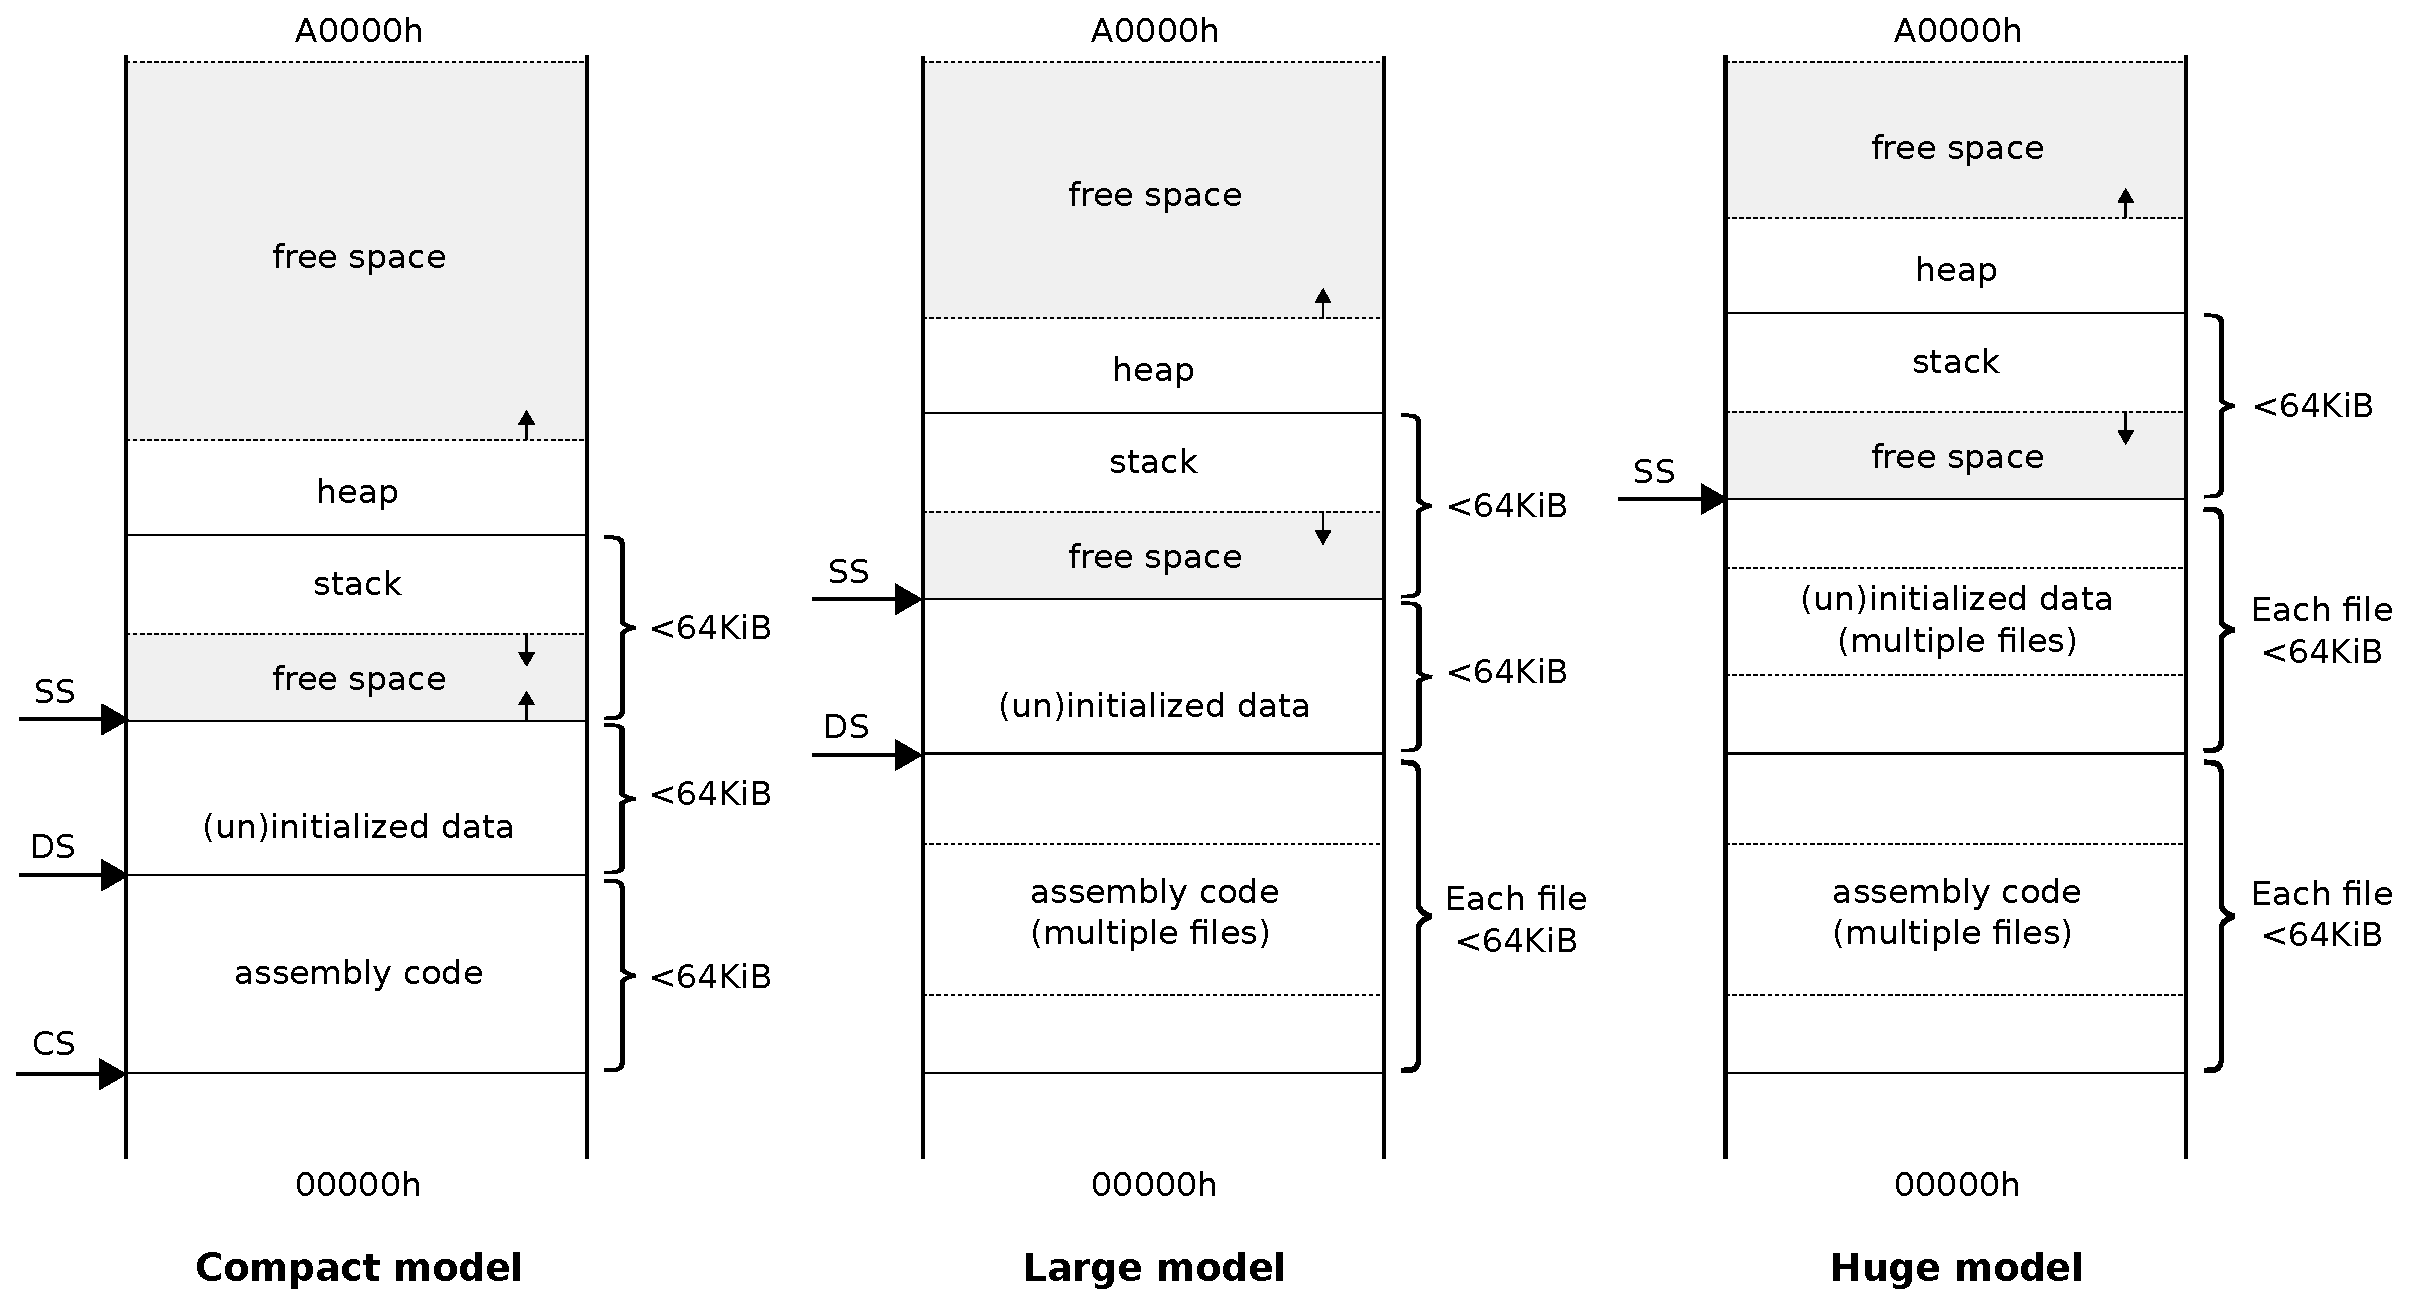
\includegraphics[width=0.8\textwidth]{imgs/drawings/memory/compact_large_huge_mm.eps}
\caption{Compact, Large and Huge memory model.}
\label{fig:mm_huge}
\end{figure}
\par

\trivia{Although the name implies differently, the huge memory model in Borland C++ is still limited to segments up to 64KiB using far pointers, and not using huge pointers. The Watcom compiler, which gained popularity in the 90's, was able to break the 64KiB segment barrier using the huge pointer reference for the huge memory model\footnote{See https://open-watcom.github.io/open-watcom-v2-wikidocs/clr.html}.}


\end{document}